% This file was converted to LaTeX by Writer2LaTeX ver. 1.0.2
% see http://writer2latex.sourceforge.net for more info
\documentclass[a4paper]{article}
\usepackage[ascii]{inputenc}
\usepackage[T1]{fontenc}
\usepackage[spanish,english]{babel}
\usepackage{amsmath}
\usepackage{amssymb,amsfonts,textcomp}
\usepackage{color}
\usepackage{array}
\usepackage{supertabular}
\usepackage{hhline}
\usepackage{hyperref}
\hypersetup{pdftex, colorlinks=true, linkcolor=blue, citecolor=blue, filecolor=blue, urlcolor=blue, pdftitle=, pdfauthor=Ruben Perez Pascual, pdfsubject=, pdfkeywords=}
\usepackage[pdftex]{graphicx}
% Outline numbering
\setcounter{secnumdepth}{3}
\renewcommand\thesection{\arabic{section}}
\renewcommand\thesubsection{\arabic{section}.\arabic{subsection}}
\renewcommand\thesubsubsection{\arabic{section}.\arabic{subsection}.\arabic{subsubsection}}
\makeatletter
\newcommand\arraybslash{\let\\\@arraycr}
\makeatother
% List styles
\newcounter{saveenum}
\newcommand\liststyleLFOxlii{%
\renewcommand\theenumi{\arabic{enumi}}
\renewcommand\labelitemi{[F0B7?]}
\renewcommand\labelenumi{\theenumi.}
\renewcommand\labelitemii{[F0A7?]}
\renewcommand\labelitemiii{[F0B7?]}
}
\newcommand\liststyleLFOxliii{%
\renewcommand\labelitemi{[F0B7?]}
\renewcommand\labelitemii{o}
\renewcommand\labelitemiii{[F0A7?]}
\renewcommand\labelitemiv{[F0B7?]}
}
\newcommand\liststyleLFOxliv{%
\renewcommand\theenumi{\arabic{enumi}}
\renewcommand\theenumii{\alph{enumii}}
\renewcommand\theenumiii{\roman{enumiii}}
\renewcommand\theenumiv{\arabic{enumiv}}
\renewcommand\labelenumi{\theenumi.}
\renewcommand\labelenumii{\theenumii.}
\renewcommand\labelenumiii{\theenumiii.}
\renewcommand\labelenumiv{\theenumiv.}
}
\newcommand\liststyleLFOxlv{%
\renewcommand\labelitemi{[F0B7?]}
\renewcommand\labelitemii{o}
\renewcommand\labelitemiii{[F0A7?]}
\renewcommand\labelitemiv{[F0B7?]}
}
\newcommand\liststyleLFOxlvi{%
\renewcommand\theenumi{\arabic{enumi}}
\renewcommand\theenumii{\alph{enumii}}
\renewcommand\theenumiii{\roman{enumiii}}
\renewcommand\theenumiv{\arabic{enumiv}}
\renewcommand\labelenumi{\theenumi.}
\renewcommand\labelenumii{\theenumii.}
\renewcommand\labelenumiii{\theenumiii.}
\renewcommand\labelenumiv{\theenumiv.}
}
% Page layout (geometry)
\setlength\voffset{-1in}
\setlength\hoffset{-1in}
\setlength\topmargin{0.4923in}
\setlength\oddsidemargin{0.9847in}
\setlength\textheight{9.7238in}
\setlength\textwidth{6.2985992in}
\setlength\footskip{0.4923in}
\setlength\headheight{0.4923in}
\setlength\headsep{0cm}
% Footnote rule
\setlength{\skip\footins}{1.1777999mm}
\renewcommand\footnoterule{\vspace*{-0.007in}\setlength\leftskip{0pt}\setlength\rightskip{0pt plus 1fil}\noindent\textcolor{black}{\rule{0.33\columnwidth}{0.007in}}\vspace*{1mm}}
% Pages styles
\makeatletter
\newcommand\ps@MP{
  \renewcommand\@oddhead{FP7-ICT-318389/DEIMOS/REPORT/CO/ GEO-Cloud-DMS-TEC-TEC15-10-E}
  \renewcommand\@evenhead{\@oddhead}
  \renewcommand\@oddfoot{}
  \renewcommand\@evenfoot{\@oddfoot}
  \renewcommand\thepage{\arabic{page}}
}
\makeatother
\pagestyle{MP}
\setlength\tabcolsep{1mm}
\renewcommand\arraystretch{1.3}
\title{}
\author{Ruben Perez Pascual}
\date{2014-07-04T11:26:00Z}
\begin{document}
\begin{flushleft}
\tablehead{}
\begin{supertabular}{llll}
\multicolumn{1}{c}{

\includegraphics[width=1.43472in,height=1.30417in]{out-img1.png} } &
\multicolumn{1}{c}{

\includegraphics[width=1.07847in,height=0.73056in]{out-img2.jpg} } &
\multicolumn{1}{c}{

\includegraphics[width=1.27847in,height=0.88681in]{out-img3.jpg} } &
\multicolumn{1}{c}{

\includegraphics[width=1.30417in,height=1.06111in]{out-img4.png} }\\
\end{supertabular}
\end{flushleft}

\bigskip


\bigskip

\begin{flushleft}
\tablehead{}
\begin{supertabular}{|m{1.98856in}|m{4.25246in}|}
\hline
Project Acronym &
\bfseries Fed4FIRE\\\hline
Project Title &
\bfseries Federation for FIRE\\\hline
Instrument &
\bfseries Large scale integrating project (IP)\\\hline
Call identifier &
\bfseries FP7-ICT-2011-8\\\hline
Project number &
\bfseries 318389\\\hline
Project website &
\bfseries www.fed4fire.eu\\\hline
Experiment &
\bfseries GEO-Cloud\\\hline
\end{supertabular}
\end{flushleft}

\bigskip


\bigskip

{\centering\bfseries
GEO-Cloud Experiment Implementation\ in Virtual Wall and BonFIRE
\par}


\bigskip

\begin{flushleft}
\tablehead{}
\begin{supertabular}{|m{1.9649599in}|m{4.27466in}|}
\hline
Work\ package &
WP10\\\hline
Task &
T10.1.2\ GEO-Cloud Experiment\\\hline
Due date &
30/05/2014\\\hline
Submission date &
09/06/2014\\\hline
Report Lead &
F\'elix Pedrera\ (DEIMOS)\\\hline
Version &
1.0\\\hline
Authors &
\selectlanguage{spanish} Manuel Jos\'e Latorre, F\'elix
Pedrera,\ Rub\'en P\'erez\ (DEIMOS)\ \\\hline
Reviewers &
Jonathan Becedas\ (DEIMOS)\\\hline
\end{supertabular}
\end{flushleft}

\bigskip


\bigskip

\begin{flushleft}
\tablehead{}
\begin{supertabular}{|m{1.9649599in}|m{4.27466in}|}
\hline
\bfseries Document ID &
\foreignlanguage{spanish}{\textbf{GEO-Cloud-DMS-TEC-TEC15-10-E}}\\\hline
Abstract &
This document provides\ technical information about\ the GEO-Cloud
experiment\ implementation\ and integration\ in Virtual Wall and
BonFIRE.\\\hline
Keywords &
Report\\\hline
\end{supertabular}
\end{flushleft}

\bigskip


\bigskip

\begin{flushleft}
\tablehead{}
\begin{supertabular}{m{1.9649599in}|m{0.31495985in}|m{3.36706in}|m{0.43505988in}|}
\hline
\multicolumn{1}{|m{1.9649599in}|}{Nature of the\ document} &
R &
Report &
X\\\hline
 &
P &
Prototype &
~
\\\hhline{~---}
 &
D &
Demonstrator &
~
\\\hhline{~---}
 &
O &
Other &
~
\\\hline
\multicolumn{1}{|m{1.9649599in}|}{Dissemination level} &
PU &
Public &
~
\\\hline
 &
PP &
Restricted to other programme participants (including the Commission) &
~
\\\hhline{~---}
 &
RE &
Restricted to a group specified by the consortium (including the
Commission) &
~
\\\hhline{~---}
 &
CO &
Confidential, only for members of the consortium (including the
Commission) &
X\\\hhline{~---}
\end{supertabular}
\end{flushleft}

\bigskip

\clearpage
\textrm{\textbf{Disclaimer}}


\bigskip

\textit{The information, documentation and figures available in this
deliverable, is written by the Fed4FIRE\ }(Federation for
FIRE)\ \textit{{}-- project consortium under EC co-financing contract
FP7-ICT-}\textit{318389}\textit{\ and does not necessarily reflect the
views of the European Commission}\textit{. The European
C}\textit{ommission is not liable for any use that may be made of the
information contained herein.}

\clearpage
\textrm{\textbf{Executive S}}\textrm{\textbf{ummary}}


\bigskip

In this document the detailed\ implementation of\ GEO-Cloud is
presented. The document is divided into the following sections:


\bigskip

In section 1, the implementation is introduced indicating the testbeds
involved in it and\ the required steps\ for the implementation.


\bigskip

Section 2 is dedicated to the implementation of the\ Space System
Simulator in\ Virtual Wall. Firstly, the new modified topology
(different to the designed one) is depicted because of the handicaps of
the hardware during the implementation. Then, nodes reservation\ is
explained and detailed. Finally, the scripts included in each type of
node are described before the presentation of the execution.


\bigskip

Section 3 is dedicated to the implementation\ of the software
developed\ in the BonFIRE testbed. Nodes reservation is firstly
depicted. Architecture and setup are also explained. And again, the
scripts for each node are included before the description of the
execution.


\bigskip

After the explanation of the implementation, the integration in\ the
testbeds is described in\ sections 4 and 5, relative\ to the
integration of Virtual Wall -- BonFIRE and BonFIRE -- IDV respectively.


\bigskip

Section 6 is devoted\ to\ describe the\ demonstration\ of the\ GEO-Cloud
experiment prepared for the European Commission in June 2014.


\bigskip

Finally, section 7 provides\ the main\ conclusions.


\bigskip

\clearpage
\textrm{\textbf{A}}\textrm{\textbf{cronyms and
A}}\textrm{\textbf{bbreviations}}


\bigskip

\begin{flushleft}
\tablehead{}
\begin{supertabular}{|m{0.8823598in}|m{5.35596in}|}
\hline
BF &
BonFIRE\\\hline
CPU &
Central Processing Unit\\\hline
CSW &
Catalogue Services for the Web\\\hline
EaaS &
Elasticity as a Service\\\hline
FTP &
File Transfer Protocol\\\hline
GS &
Ground Station\\\hline
HTTP &
Hypertext Transfer Protocol\\\hline
Sat &
Satellite\\\hline
SQL &
Structured Query Language\\\hline
VM &
Virtual Machine\\\hline
VW &
Virtual Wall\\\hline
WMS &
Web Map Service\\\hline
WMS-C &
Web Map Tile Caching\\\hline
WMTS &
Web Map Tile Service\\\hline
WPS &
Web Processing Service\\\hline
WS &
Web Service\\\hline
XML &
eXtensible Markup Language\\\hline
\end{supertabular}
\end{flushleft}
\clearpage
\textrm{\textbf{Table of C}}\textrm{\textbf{ontents}}


\bigskip

\setcounter{tocdepth}{3}
\tableofcontents

\bigskip

\section[Introduction]{Introduction}
\hypertarget{Toc390097010}{}
\bigskip

The GEO-Cloud experiment\ implementation\ is the following step in the
project, after the design of the system. This step consists of the
procedures to be followed in order to have the testbeds available and
ready to execute the experiment and start obtaining results. In the
document, the whole implementation process is covered and also the
integration between testbeds is explained.


\bigskip

Besides, a demonstration of the project was required by the European
Commission to know first-hand how it works. It is presented the
execution of one scenario together with a video that provides visual
information of the satellite system in the process, and also including
an interactive exercise allowing the access to the images acquired
during the demonstration through a web service.

\section[Implementation in Virtual Wall]{Implementation in Virtual Wall}
\hypertarget{Toc390097011}{}
\bigskip

In Virtual Wall the Space System Simulator was implemented. It is
constituted of the following modules:

\liststyleLFOxlii
\begin{itemize}
\item The\ \textit{Satellite System Simulator}
\item The\ \textit{Ground Station System Simulator}
\end{itemize}

\bigskip

The topology network designed is depicted in\ Figure 1.


\bigskip

{\centering 
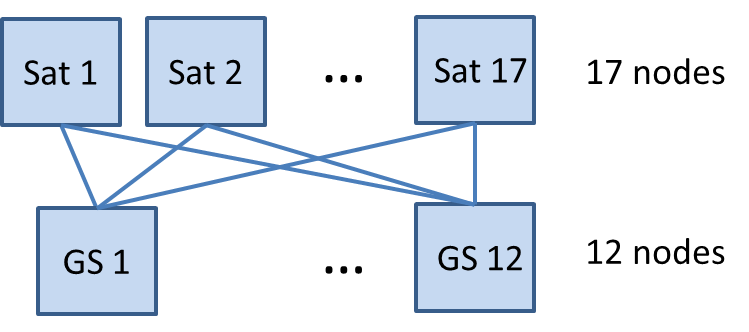
\includegraphics[width=3.08108in,height=1.36551in]{out-img5.png} \par}

{\centering\bfseries
\label{bkm:Ref390072131}Figure\ 1\ Topology Network in Virtual Wall
\par}


\bigskip

The previous topology network involves Sat nodes to have 12 connections
with the GS nodes; and GS nodes 17 connections with Sat nodes plus one
connection with the BonFIRE cloud.


\bigskip

The nodes in Virtual Wall have a limitation of 5 physical connections.
To deploy the previous topology we adapted the Space System Simulator
software to establish those connections by software. This was done by
making the Satellite System Simulator flexible to connect with any
ground station from GS1 to GS12. Then the Satellite System Simulator
can be multiplied and only connect to it the number of GS nodes
desired.\ 


\bigskip

The solution was to multiply the Satellite System Simulator by three and
connect 4 ground stations to each Satellite System Simulator. This
ensures the same performance and dynamics of the previous topology
network described in\ Figure 1, and the only thing it changes is the
software.


\bigskip

The Space System Simulator implemented in Virtual Wall is depicted
in\ Figure 2.

{\centering 
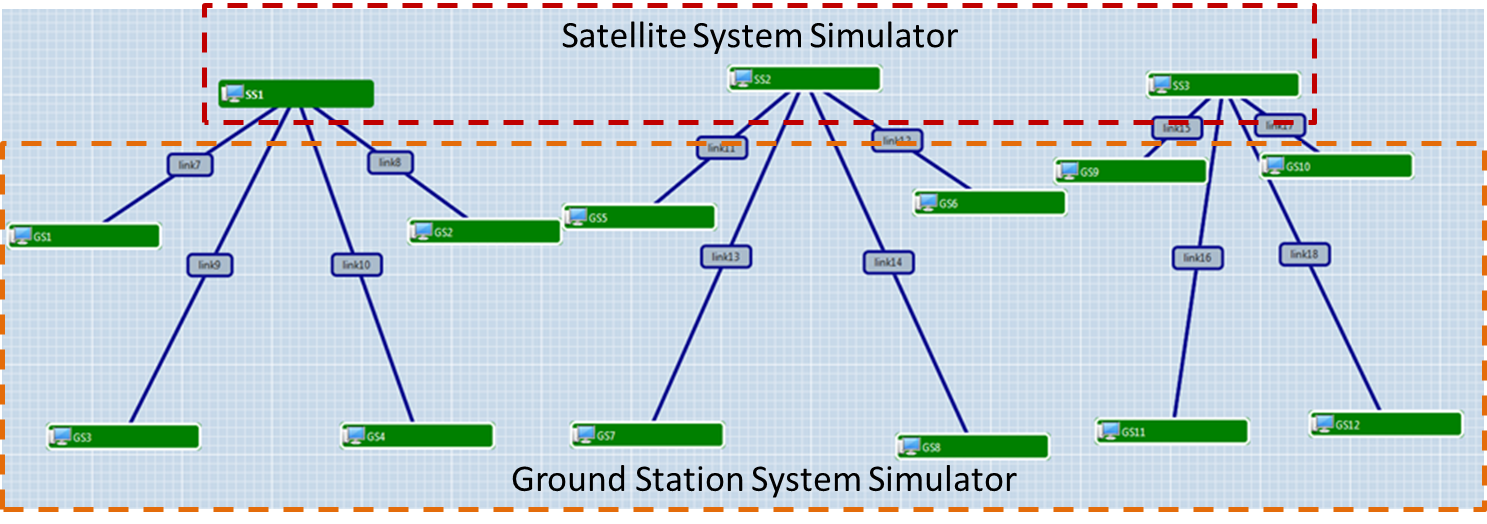
\includegraphics[width=6.44403in,height=2.27094in]{out-img6.png} \par}

{\centering\bfseries
\label{bkm:Ref390072850}Figure\ 2\ Space System Simulator implemented in
Virtual Wall
\par}


\bigskip

\subsection[Nodes reservation\ and\ setup]{Nodes
reservation\ and\ setup}
\hypertarget{Toc390097012}{}The Space System Simulator is then
constituted by 15\ {\textquotedblleft}Generic
nodes{\textquotedblright}\ in Virtual Wall 1. The configuration of the
experiment makes the provisioning of\ {\textquotedblleft}any available
node{\textquotedblright}, which is more flexible in case a node is
being used in other experiment\ (see\ Figure 3).\ The links
between\ SS\ (Satellite Simulators)\ and GS\ (Ground Stations
Simulators)\ nodes are TCP.\ The definition of the dependencies and the
commands that will be installed at setup is defined in JFed using a
RSPEC specification. This specification includes some bash commands or
instructions that will execute after reservation automatically.


\bigskip

{\centering 
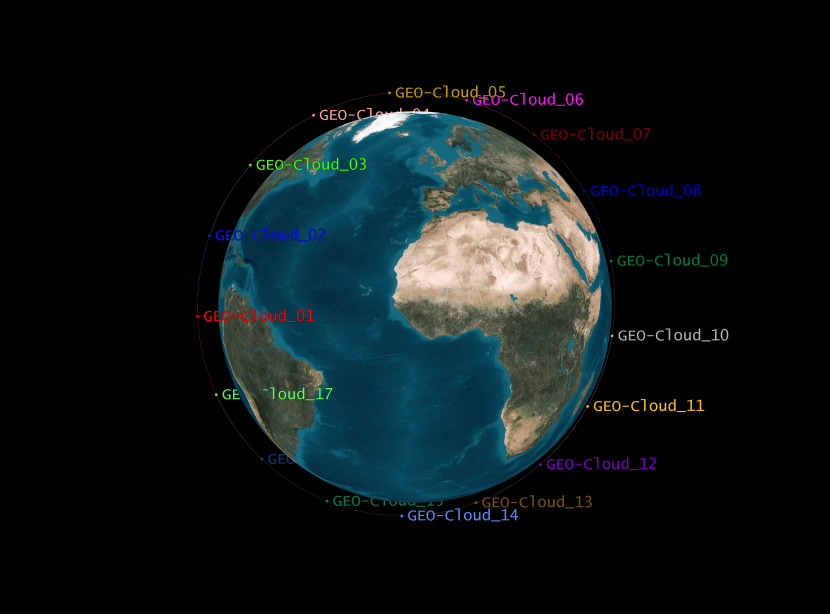
\includegraphics[width=2.97835in,height=3.15141in]{out-img7.png} \par}

{\centering\bfseries
\label{bkm:Ref390077695}Figure\ 3\ Configuration of Virtual Wall nodes
\par}

\subsubsection[SS\ nodes\ setup]{SS\ nodes\ setup}
\hypertarget{Toc390097013}{}
\bigskip

The configuration of the nodes is done by using JFed Experiment.\ The
Satellite Simulators software is developed under Python. To install the
libraries the nodes need connectivity with the Internet. For that
purpose a gateway has to be configured:


\bigskip

{\itshape
{\textless}execute shell={\textquotedbl}sh{\textquotedbl}
command={\textquotedbl}sudo route del default gw
10.2.15.254{\textquotedbl}/{\textgreater}}

{\itshape
{\textless}execute shell={\textquotedbl}sh{\textquotedbl}
command={\textquotedbl}sudo route add default gw
10.2.15.253{\textquotedbl}/{\textgreater}}


\bigskip

And the update of the system has to be carried out to update the
repositories and dependencies:


\bigskip

{\itshape
{\textless}execute shell={\textquotedbl}sh{\textquotedbl}
command={\textquotedbl}sudo apt-get
update{\textquotedbl}/{\textgreater}}


\bigskip

Once the update is finished Python can be installed. The Satellite
Simulators require the connection with a database that provides the
scenario number and the initial conditions for their execution. The
MySQL library is also required:


\bigskip

{\itshape
{\textless}execute shell={\textquotedbl}sh{\textquotedbl}
command={\textquotedbl}sudo apt-get install python python-mysqldb
-y{\textquotedbl}/{\textgreater}}


\bigskip

The database is located in BonFIRE. It has an IP that can change. In
order to obtain that IP and include it in the Satellite Simulator, a
script to acquire the IP of the database was developed
{\textquotedblleft}\textit{push\_dbIP.sh}{\textquotedblright}.\ \ It
contains the following code:


\bigskip

{\ttfamily
\#!/bin/bash}


\bigskip

{\ttfamily
ip=\$1}


\bigskip

{\ttfamily
touch /users/jbecedas/ipdb}

\texttt{echo \$ip {\textgreater} /users/jbecedas/ipdb}


\bigskip

This file is located in Google Drive. The following sentence acquires
the file from Google Drive:


\bigskip

\textit{{\textless}execute shell={\textquotedbl}sh{\textquotedbl}
command={\textquotedbl}sudo wget
-{}-no-check-certificate\ }\textit{\textcolor[rgb]{0.7529412,0.0,0.0}{google\_drive\_host\_address}}\textit{\ }\textit{{}-O
/users/jbecedas/push\_dbIP.sh{\textquotedbl}/{\textgreater}}


\bigskip

Where\ \textit{\textcolor[rgb]{0.7529412,0.0,0.0}{google\_drive\_host\_address}}\textit{\textcolor[rgb]{0.7529412,0.0,0.0}{\ }}is
the address of the Google Drive host in which the scripts are located.


\bigskip

The execution of the push\_dbIP.sh script acquires the IP of the
database and includes it in the file\ ipdb, created by
{\textquotedblleft}\textit{push\_dbIP.sh}{\textquotedblright}:

{\textless}execute shell={\textquotedbl}sh{\textquotedbl}
command={\textquotedbl}sudo bash /users/jbecedas/push\_dbIP.sh
129.215.175.147{\textquotedbl}/{\textgreater}


\bigskip

Now, the node is perfectly configured to proceed with the installation
of the Satellite Simulator. The software of the simulator has been
archived\ too\ in Google Drive. With the following command the software
is acquired:


\bigskip

\textit{{\textless}execute shell={\textquotedbl}sh{\textquotedbl}
command={\textquotedbl}sudo wget
-{}-no-check-certificate\ }\textit{\textcolor[rgb]{0.7529412,0.0,0.0}{google\_drive\_host\_address}}\textit{\ }\textit{{}-O
/users/jbecedas/satellite.py{\textquotedbl}/{\textgreater}}


\bigskip

It can now be executed in the node.


\bigskip

\subsubsection[GS nodes\ setup]{GS nodes\ setup}
\hypertarget{Toc390097014}{}
\bigskip

The\ Ground Station Simulators software is developed under Python. To
install the libraries the nodes need connectivity with the Internet.
For that purpose a gateway has to be configured:


\bigskip

{\itshape
{\textless}execute shell={\textquotedbl}sh{\textquotedbl}
command={\textquotedbl}sudo route del default gw
10.2.15.254{\textquotedbl}/{\textgreater}\newline
{\textless}execute shell={\textquotedbl}sh{\textquotedbl}
command={\textquotedbl}sudo route add default gw
10.2.15.253{\textquotedbl}/{\textgreater}}

As occurred with the SS nodes, the update and the installation of Python
and MySQL are required:


\bigskip

\textit{{\textless}execute shell={\textquotedbl}sh{\textquotedbl}
command={\textquotedbl}sudo apt-get
update{\textquotedbl}/{\textgreater}}\textit{\newline
\ {\textless}execute shell={\textquotedbl}sh{\textquotedbl}
command={\textquotedbl}sudo apt-get install python python-mysqldb
-y{\textquotedbl}/{\textgreater}}


\bigskip

The IP of the database has to be included in the node:


\bigskip

\textit{{\textless}execute shell={\textquotedbl}sh{\textquotedbl}
command={\textquotedbl}sudo wget
-{}-no-check-certificate\ }\textit{\textcolor[rgb]{0.7529412,0.0,0.0}{google\_drive\_host\_address}}\textit{\ }\textit{{}-O
/users/jbecedas/push\_dbIP.sh{\textquotedbl}/{\textgreater}}\textit{\newline
{\textless}execute shell={\textquotedbl}sh{\textquotedbl}
command={\textquotedbl}sudo bash /users/jbecedas/push\_dbIP.sh
129.215.175.147{\textquotedbl}/{\textgreater}}


\bigskip

The software\ of the Ground Stations Simulator\ developed in Python is
also located in Google Drive:


\bigskip

\textit{{\textless}execute shell={\textquotedbl}sh{\textquotedbl}
command={\textquotedbl}sudo wget
-{}-no-check-certificate\ }\textit{\textcolor[rgb]{0.7529412,0.0,0.0}{google\_drive\_host\_address}}\textit{\ }\textit{\ }\textit{{}-O
/users/jbecedas/groundstation.py{\textquotedbl}/{\textgreater}}


\bigskip

The GS nodes are required to open an FTP to be accessed from the
Orchestrator in BonFIRE. The FTP is configured by executing the
{\textquotedblleft}install\_ftp.sh{\textquotedblright} file. This file
has the following code:


\bigskip

{\ttfamily
\#!/bin/bash}


\bigskip

{\ttfamily
sudo apt-get update}

{\ttfamily
sudo apt-get install mysql-client ftp ftplib3 vsftpd -y}

{\ttfamily
sudo sed -i {\textquotedbl}s/listen=YES/listen=NO/{\textquotedbl}
/etc/vsftpd.conf}

{\ttfamily
sudo sed -i
{\textquotedbl}s/\#listen\_ipv6=NO/listen\_ipv6=YES/{\textquotedbl}
/etc/vsftpd.conf}

{\ttfamily
sudo sed -i
{\textquotedbl}s/\#listen\_ipv6=YES/listen\_ipv6=YES/{\textquotedbl}
/etc/vsftpd.conf}

{\ttfamily
sudo sed -i
{\textquotedbl}s/anonymous\_enable=YES/anonymous\_enable=NO/{\textquotedbl}
/etc/vsftpd.conf}

{\ttfamily
sudo sed -i
{\textquotedbl}s/\#local\_enable=NO/local\_enable=YES/{\textquotedbl}
/etc/vsftpd.conf}

{\ttfamily
sudo sed -i
{\textquotedbl}s/\#local\_enable=YES/local\_enable=YES/{\textquotedbl}
/etc/vsftpd.conf}

{\ttfamily
sudo sed -i
{\textquotedbl}s/\#write\_enable=NO/write\_enable=YES/{\textquotedbl}
/etc/vsftpd.conf}

{\ttfamily
sudo sed -i
{\textquotedbl}s/\#write\_enable=YES/write\_enable=YES/{\textquotedbl}
/etc/vsftpd.conf}

{\ttfamily
sudo sed -i {\textquotedbl}s/\#local\_umask/local\_umask/{\textquotedbl}
/etc/vsftpd.conf}

{\ttfamily
sudo sed -i
{\textquotedbl}s/\#chroot\_list\_file/chroot\_list\_file/{\textquotedbl}
/etc/vsftpd.conf}

{\ttfamily
sudo mkdir -p /home/ftp/deimos}

{\selectlanguage{spanish}\ttfamily
sudo mkdir /home/deimos}

{\selectlanguage{spanish}\ttfamily
sudo useradd -d /home/deimos -g ftp \ deimos}

{\ttfamily
sudo chmod 777 -R /home}

{\ttfamily
sudo touch /etc/vsftpd.chroot\_list}

{\selectlanguage{spanish}\ttfamily
sudo su}

{\selectlanguage{spanish}\ttfamily
echo {\textquotedbl}deimos:deimos{\textquotedbl}{\textbar}chpasswd}

{\selectlanguage{spanish}\ttfamily
echo {\textquotedbl}deimos{\textquotedbl} {\textgreater}{\textgreater}
/etc/vsftpd.chroot\_list}

{\ttfamily
sudo service vsftpd restart}


\bigskip

It is executed as follows:


\bigskip

{\itshape
{\textless}execute shell={\textquotedbl}sh{\textquotedbl}
command={\textquotedbl}sudo bash
/users/jbecedas/install\_ftp.sh{\textquotedbl}/{\textgreater}}


\bigskip

Through the FTP connection the raw data will be transferred from the GS
nodes to the BonFIRE cloud.\ The raw data is located in Google Drive
too.


\bigskip

\textit{{\textless}execute shell={\textquotedbl}sh{\textquotedbl}
command={\textquotedbl}sudo wget
-{}-no-check-certificate\ }\textit{\textcolor[rgb]{0.7529412,0.0,0.0}{google\_drive\_host\_address}}\textit{\textcolor[rgb]{0.7529412,0.0,0.0}{\ }}\textit{{}-O\ }\textit{/tmp/original.bin
{\textquotedbl}/{\textgreater}}\newline


\subsection[Execution]{Execution}
\hypertarget{Toc390097015}{}
\bigskip

The execution of the Satellite Simulators and the Ground Station
Simulators is described
in\ GEO-Cloud-DMS-TEC-TEC11-10-E-2014-05-07.docx.\ 


\bigskip

A summary is here included:


\bigskip

The execution of the Satellite Simulator software:

{\itshape
{\textgreater} python satellite.py {\textless}IDSAT{\textgreater}
{\textless}SCENARIO{\textgreater} {\textless}DBHOST{\textgreater}
[LOGLEVEL]}

where:

\liststyleLFOxliii
\begin{itemize}
\item IDSAT is the satellite identity. This value must be an integer.\ 
\item SCENARIO is the scenario number to simulate. Must be an integer.
\item DBHOST is the host where the data base is located. Must be a
hostname or an IP direction.
\item LOGLEVEL is the level of log that the software will show. The
values can be: INFO, DEBUG. This parameter is optative. By default its
value is INFO.\ 
\end{itemize}
The execution of the Ground Station Simulator software:

{\itshape
{\textgreater} python groundstation.py {\textless}IDSAT{\textgreater}
{\textless}SCENARIO{\textgreater} {\textless}DBHOST{\textgreater}
[LOGLEVEL]}

where:

\liststyleLFOxliii
\begin{itemize}
\item IDSAT is the ground station identity. This value must be an
integer.\ 
\item SCENARIO is the scenario to simulate. Must be an integer.
\item DBHOST is the host where the data base is located. Must be a
hostname or an IP direction.
\item LOGLEVEL is the level of log that the software will show. The
values can be: INFO, DEBUG. This parameter is optative. By default its
value is INFO.\ 
\end{itemize}

\bigskip

\section[Implementation in\ BonFIRE]{Implementation in\ BonFIRE}
\hypertarget{Toc390097016}{}
\bigskip

In BonFIRE the following modules are computed:\ 

\liststyleLFOxliv
\setcounter{saveenum}{\value{enumi}}
\begin{enumerate}
\setcounter{enumi}{\value{saveenum}}
\item The distributed database with the information of the scenario and
the initial conditions for the experiment.
\item Orchestrator
\item Image Processing Chain.
\item Archive and Catalogue.
\item Image Distribution and Visualization.\ \ 
\end{enumerate}
\subsection[Nodes reservation]{Nodes reservation}
\hypertarget{Toc390097017}{}\subsubsection[Distributed
Database]{Distributed Database}
\hypertarget{Toc390097018}{}It is a Virtual Machine\ instance type
medium, with 2 CPUs, 2048 MiB in the\ INRIA\ testbed.\ It was
configured to have an IPV4.

\subsubsection[Orchestrator]{Orchestrator}
\hypertarget{Toc390097019}{}It is an x-large instance with 4 CPUs, 8192
MiB, in the EPCC testbed.

\subsubsection[Processing Chain]{Processing Chain}
\hypertarget{Toc390097020}{}It is an x-large instance with 4 CPUs, 8192
MiB, in the EPCC testbed.\ 


\bigskip

It has a Datablock linked with 100GB of memory.

\subsubsection[Archive and Catalogue]{Archive and Catalogue}
\hypertarget{Toc390097021}{}It is a Virtual Machine instance type
medium, with 2CPUs, 2048 MiB in the INRIA testbed.\ It was configured
to have an IPV4.


\bigskip

It has a Datablock linked with 100GB of memory.\ 

\subsubsection[Image Distribution and Visualization]{Image Distribution
and Visualization}
\hypertarget{Toc390097022}{}It is constituted by:

\liststyleLFOxlv
\begin{itemize}
\item Raster and Vector Datastore: It is a Virtual Machine Custom\ in
INRIA. It is linked an R\&V Datastore, which is a shared storage
instance with 100GB located in be-ibbt.\ 
\item EO server: It is a Virtual Machine Custom\ in INRIA. \ It was
configured to have an IPV4
\item Tiles Cache: It is a Virtual Machine Custom in INRIA. It was
configured to have an IPV4. It is linked an R\&V Datastore, which is a
shared storage instance with 100GB located in be-ibbt.
\end{itemize}
\subsection[Nodes\ setup]{Nodes\ setup}
\hypertarget{Toc390097023}{}\subsubsection[Database
node\ setup]{Database node\ setup}
\hypertarget{Toc390097024}{}The software of the database\ creation and
filling the database\ is developed in Python.\ The file
{\textquotedblleft}setup.sh{\textquotedblright}\ in the database
folder\ contains the\ setup of\ the node.


\bigskip

The node is firstly updated and upgraded:


\bigskip

{\itshape
apt-get update}

{\itshape
apt-get upgrade -y}


\bigskip

Then, the libraries of\ Python,\ MySQL server, MySQL client, and
essentials tools\ are installed:


\bigskip

{\itshape
apt-get install mysql-server -y}

{\itshape
apt-get install build-essential python-dev libmysqlclient-dev -y}

{\itshape
apt-get install python-mysqldb}


\bigskip

The service MySQL is restarted, just in case it was started before:


\bigskip

{\itshape
service mysql restart}


\bigskip

The database {\textquotedblleft}modelDataBase{\textquotedblright} is
incorporated to MySQL:


\bigskip

{\itshape
mysql -u root -p {\textless} modelDataBase}


\bigskip

The database {\textquotedblleft}modelDataBase{\textquotedblright} is
computed in the
file\ {\textquotedblleft}modelDataBase{\textquotedblright}.\ It is
constituted of three tables: GroundStations, Scenarios and Satellites.
The database is described
in\ GEO-Cloud-DMS-TEC-TEC11-10-E-2014-05-07.docx.\ 


\bigskip

Then, a bind is done in the public interface:


\bigskip

{\itshape
sed {\textquotedbl}s/bind-address/bind-address \$(hostname -I {\textbar}
cut -f 1 -d {\textquotesingle} {\textquotesingle}) \#/g{\textquotedbl}
/etc/mysql/my.cnf}


\bigskip

And, finally, the service Mysql is restarted to update the previous
configuration:


\bigskip

{\itshape
service mysql restart}


\bigskip

\subsubsection[Orchestrator node setup]{Orchestrator node setup}
\hypertarget{Toc390097025}{}The software of the Orchestrator is
developed in Python. The file
{\textquotedblleft}setup.sh{\textquotedblright} in the orchestrator
folder contains the setup of the node.


\bigskip

The node is firstly updated and upgraded:


\bigskip

{\itshape
apt-get update}

{\itshape
apt-get upgrade -y}


\bigskip

Then, the libraries of Python, MySQL Python client, Python ftp to
connect with the ground stations, and other ftp libraries:

{\itshape
apt-get install python-mysqldb python-ftputil ftplib-dev ftplib3}


\bigskip

After that,\ a pair of rsa-keys has to be generated. These are\ created
by\ doing the following:\ 


\bigskip

{\itshape
ssh-keygen --t rsa\ }


\bigskip

This generates two files into the directory \~{}/.ssh,\ which are named
id\_rsa.pub and id\_rsa. The first one is the public key which has to
be copied into the remote machine to\ allow\ remote access; the second
one is the private key, but this file does not need
any\ further\ modifications.\ 


\bigskip

Then the code of the orchestrator is uploaded to the node and the
main.py is executed:


\bigskip

{\itshape
python main.py}


\bigskip

More information about the orchestrator code can be found
in\ GEO-Cloud-DMS-TEC-TEC10-10-E-2014-03-10.

\subsubsection[Processing Chain node setup]{Processing Chain node setup}
\hypertarget{Toc390097026}{}The node of the processing chain was setup
to install the image processing software previously developed by
Elecnor Deimos. Both the setup and the installation of the image
processing software are background of Elecnor Deimos. They are
described in the internal report\ D2-DMS-PP-TEC-SIM05-2C.pdf


\bigskip

Once the setup is\ ready, the public key of the Orchestrator node has to
be copied into the file \ \~{}/.ssh/known\_hosts\ to allow
the\ Orchestrator\ to\ establish a remote connection using ssh\ and
scp.\ In this\ node a pair of\ rsa-keys has to be generated\ too. To
generate them,\ the following command is executed.


\bigskip

{\itshape
ssh-keygen --t rsa\ }


\bigskip

\subsubsection[Archive and Catalogue node setup]{Archive and Catalogue
node setup}
\hypertarget{Toc390097027}{}The archive and catalogue software is based
on the open geo-software Geoserver. It requires Java and Apache-Tomcat.


\bigskip

The node is configured with the Geoserver version 2.5 and ApacheTomcat
7.0.53. The configuration of the node and the installation of the
software required are computed in the file install.sh.


\bigskip

The node is updated and upgraded:


\bigskip

{\itshape
apt-get update \&\& apt-get upgrade -y}


\bigskip

Unzip, Wget and Java dependencies are installed:


\bigskip

{\itshape
apt-get install unzip wget openjdk-6-jdk openjdk-6-jre -y}


\bigskip

Then, Apache-Tomcat, Geoserver and the Geoserver plugin are installed
and configured.\ 


\bigskip

{\itshape
cd /tmp}

{\itshape
rm -rf /tmp/geo* /tmp/apache* /usr/share/tomcat* /tmp/*.jar}

{\itshape
wget -{}-tries=10
downloads.sourceforge.net/project/geoserver/GeoServer/\$\{VERSIONGS\}/\$WAR\&\&
unzip \$\{WAR\} \&\& rm \$\{WAR\}}

{\itshape
wget -{}-tries=10
apache.rediris.es/tomcat/tomcat-7/v\$\{VERSIONT\}/bin/\$\{APACHE\}.tar.gz
\&\& tar xvzf \ \$\{APACHE\}.tar.gz\ }

{\itshape
wget -{}-tries=10
http://sourceforge.net/projects/geoserver/files/{\textquotedbl}GeoServer
Extensions{\textquotedbl}/\$\{VERSIONGS\}/\$\{PLUGIN\} \&\& unzip
\$\{PLUGIN\} \&\& rm \$\{PLUGIN\}}

{\itshape
\#http://downloads.sourceforge.net/project/geoserver/GeoServer\%20Extensions/\$\{VERSIONGS\}/\$\{PLUGIN\}?r=http\%3A\%2F\%2Fsourceforge.net\%2Fprojects\%2Fgeoserver\%2Ffiles\%2FGeoServer\%2520Extensions\%2F2.5\%2F\&ts=1399541643\&use\_mirror=kent}

{\itshape
export CATALINA\_HOME=/usr/share/tomcat7/\$\{APACHE\}/}

{\itshape
export JAVA\_OPTS={\textquotedbl}-Xms1024m -Xmx10246m -XX:NewSize=256m
-XX:MaxNewSize=356m -XX:PermSize=256m
-XX:MaxPermSize=356m{\textquotedbl}}


\bigskip


\bigskip

{\itshape
JAVA\_HOME=/usr/lib/jvm/java-1.6.0-openjdk}

{\itshape
JRE\_HOME=/usr/lib/jvm/java-1.6.0-openjdk/jre}

{\itshape
\#export JAVA\_HOME}

{\itshape
\#export JRE\_HOME}

{\itshape
PATH=\$PATH:\$JAVA\_HOME/bin:\$JRE\_HOME/bin}

{\itshape
export PATH}


\bigskip

{\itshape
mkdir /usr/share/tomcat7}

{\itshape
mv /tmp/\$\{APACHE\} /usr/share/tomcat7}


\bigskip

{\itshape
sed -i
{\textquotesingle}s/{\textquotedbl}8080{\textquotedbl}/{\textquotedbl}80{\textquotedbl}/g{\textquotesingle}
/usr/share/tomcat7/\$\{APACHE\}/conf/server.xml}


\bigskip

{\itshape
mv /tmp/geoserver.war /usr/share/tomcat7/\$\{APACHE\}/webapps}

{\itshape
sleep 2s}


\bigskip

{\itshape
/usr/share/tomcat7/\$\{APACHE\}/bin/startup.sh}

{\itshape
\#/usr/share/tomcat7/\$\{APACHE\}/bin/startup.sh}


\bigskip

{\itshape
sleep 2s}


\bigskip

{\itshape
mv /tmp/*.jar
/usr/share/tomcat7/apache-tomcat-7.0.53/webapps/geoserver/WEB-INF/lib/}


\bigskip

{\itshape
\#/usr/share/tomcat7/\$\{APACHE\}/bin/stop.sh}

{\itshape
/usr/share/tomcat7/\$\{APACHE\}/bin/startup.sh}


\bigskip

Finally, the RSA public key from the Processing chain node has to be
copied into the \~{}/.ssh/known\_hosts file\ to allow the\ Processing
chain node\ to\ establish a remote connection using ssh and scp.

\subsubsection[Image Distribution and Visualization nodes\ setup]{Image
Distribution and Visualization nodes\ setup}
\hypertarget{Toc390097028}{}
\bigskip


\bigskip

\subsection[Architecture]{Architecture}
\hypertarget{Toc390097029}{}
\bigskip

The architecture of the system computed in cloud is depicted in\ Figure
4.\ The communications between modules and other testbeds are also
depicted.\ 


\bigskip


\bigskip

{\centering 
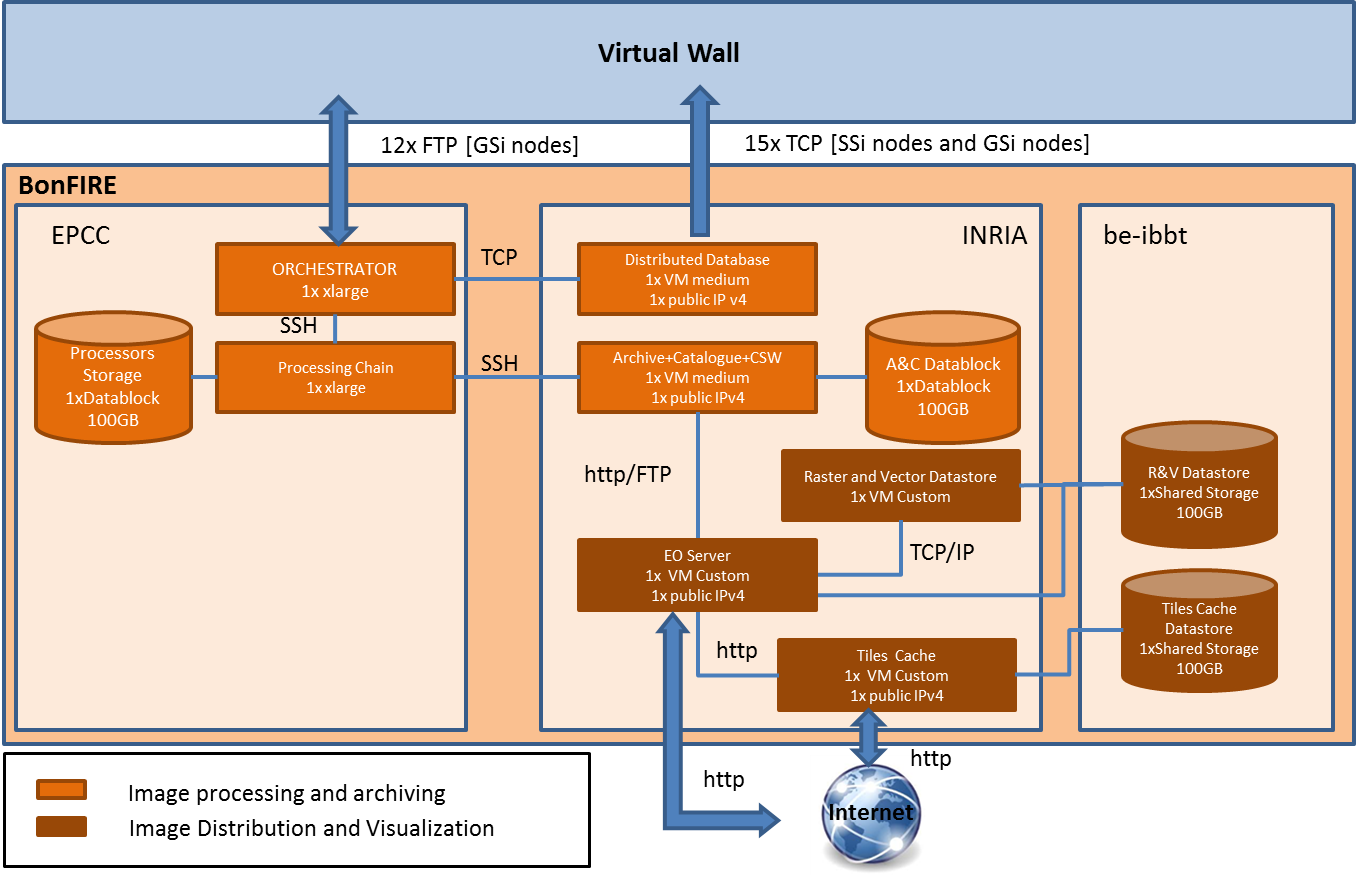
\includegraphics[width=6.22779in,height=4.01872in]{out-img8.png} \par}


\bigskip

{\centering\bfseries
\label{bkm:Ref390088635}Figure\ 4\ Architecture of the system computed
in cloud
\par}


\bigskip

The previous architecture\ makes the Orchestrator and the Processing
Chain work slightly different to the functioning designed
in\ GEO-Cloud-DMS-TEC-TEC10-10-E-2014-03-10.docx. Note that here; the
orchestrator does not communicated with a shared storage, in which the
processors send the products and from which the A\&C module gets the
final product. On the contrary, there is a Storage instance associated
to the Processing Chain. This is a temporal solution while the Fed4FIRE
partners are developing the Elasticity as a Service characteristic for
BonFIRE.\ 


\bigskip

We will start obtaining preliminary results with this solution and when
the Elasticity as a Service is ready we will change the architecture
for the originally designed one, in order to use the elasticity
feature.


\bigskip


\bigskip

\section{GEO-Cloud demo}

\bigskip

A demo of the GEO-Cloud experiment was prepared to be presented to the
European Commission during the first Fed4FIRE review.\ The demo
consists of executing the GEO-Cloud experiment to measure the time it
takes an image from its download in a ground station until a\ user
accesses to it through the Internet.\ Figure 5\ depicts the
architecture of the GEO-Cloud system and its functionality.


\bigskip


\bigskip

 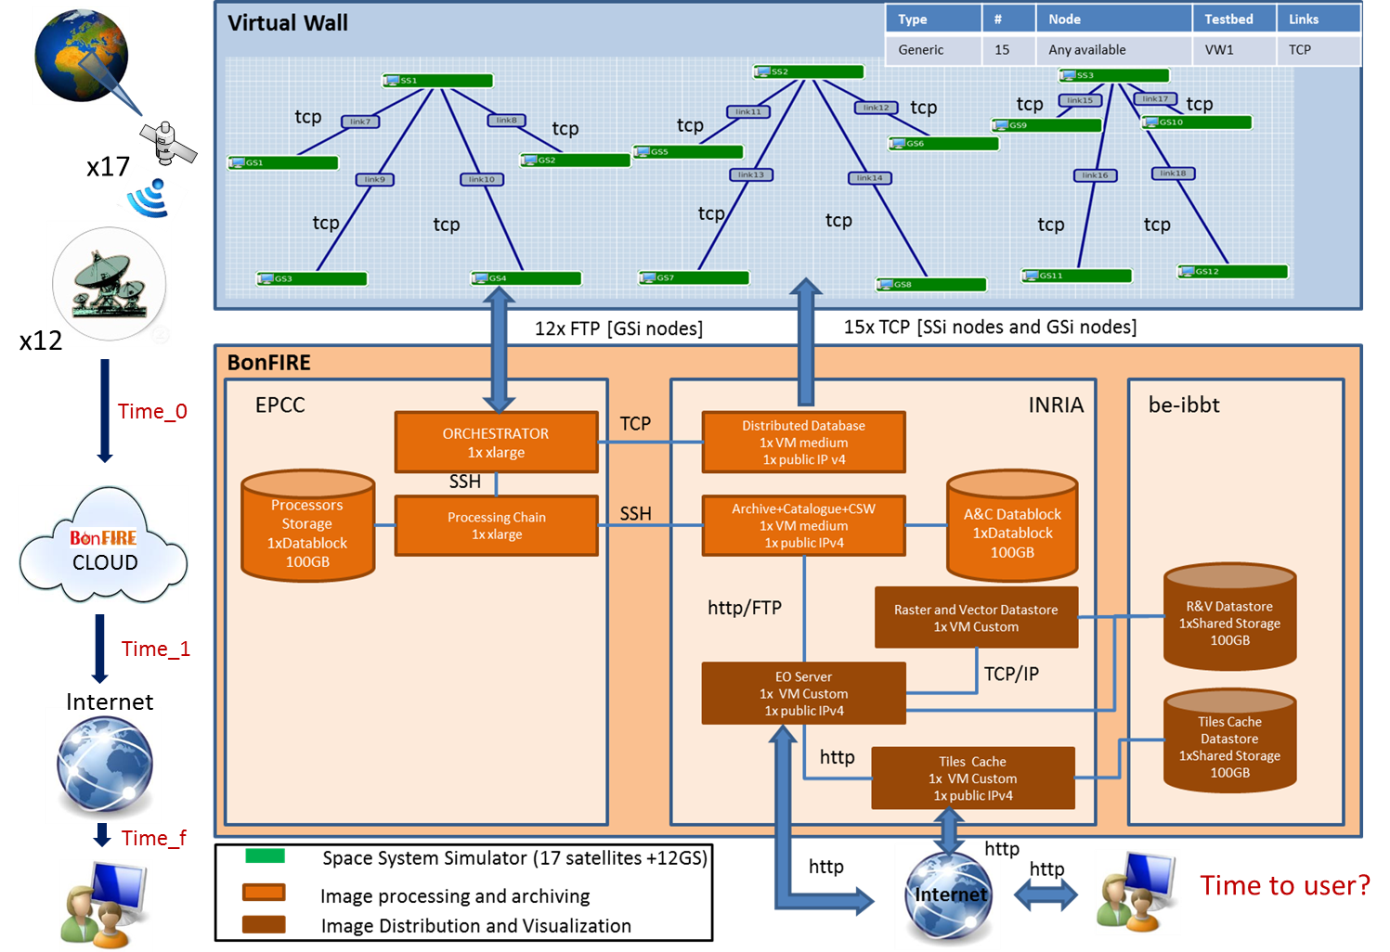
\includegraphics[width=6.31226in,height=4.32617in]{out-img9.png} 

{\centering\bfseries
\label{bkm:Ref390096338}Figure\ 5\ GEO-Cloud demo
\par}


\bigskip

Table 1\ summarizes the actions\ that will be carried out in the
GEO-Cloud demo.\ 

{\centering\bfseries
\label{bkm:Ref390096557}Table\ 1\ Actions of the GEO-Cloud demo
\par}

 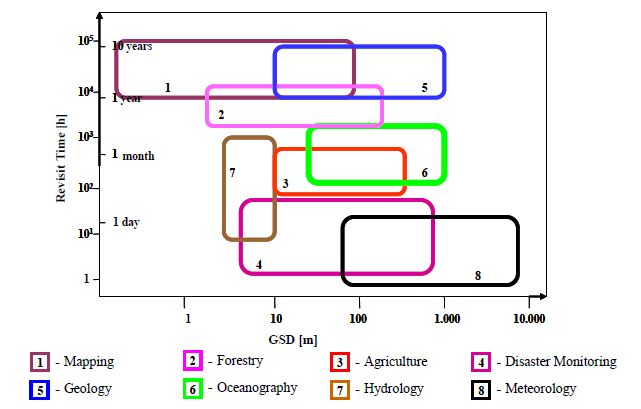
\includegraphics[width=6.28372in,height=4.23585in]{out-img10.png} 

\section[Conclusions]{Conclusions}
\hypertarget{Toc390097031}{}
\bigskip

This document presents the implementation and integration of all the
modules that constitute the GEO-Cloud system.\ We can say that the
first release of the GEO-Cloud experiment is ready. However some future
works will be carried out during the experiment execution stage:


\bigskip

\liststyleLFOxlvi
\setcounter{saveenum}{\value{enumi}}
\begin{enumerate}
\setcounter{enumi}{\value{saveenum}}
\item Implementation of the original architecture when the Elasticity as
a Service will be ready in BonFIRE.
\item Setup of the\ impairments in the Virtual Wall networks.
\end{enumerate}

\bigskip


\bigskip


\bigskip
\end{document}
